\documentclass[final,hyperref={pdfpagelabels=false}]{beamer}
\usepackage[orientation=portrait,width=54,height=70,scale=1.4]{beamerposter}
\usepackage{graphicx}
\usepackage{tikz}
\usepackage{macros/wfu-poster} % modified Aachen theme.
\usepackage{amsmath}
\usepackage{calc}
\usepackage{amssymb}
\usepackage{xcolor}
\usepackage{graphicx}


\title{Searching for Cyclic-Invariant Fast Matrix Multiplication Algorithms}
\author{João Pinheiro, Grey Ballard, Frank Moore}
\institute{Department of Computer Science}
\date{October 18, 2023}

\begin{document}
\begin{frame}[t]
% Use the title box template
% \usebeamertemplate*{headline}

% Create poster layout here
\begin{columns}[t]
    \begin{column}{.5\linewidth}
        \begin{block}{Searching for Fast Matrix Multiplication Algorithms}
        \textbf{Classical Matrix Multiplication:}
            \begin{equation*}
                \begin{bmatrix}
                    A_{11} & A_{12}\\
                    A_{21} & A_{22}
                \end{bmatrix}
                \begin{bmatrix}
                    B_{11} & B_{12}\\
                    B_{21} & B_{22}
                \end{bmatrix}
                =
                \begin{bmatrix}
                    A_{11}B_{11} + A_{12}B_{21} &\ & A_{11}B_{12} + A_{12}B_{22}\\
                    A_{21}B_{11} + A_{22}B_{21} &\ & A_{21}B_{12} + A_{22}B_{22}
                \end{bmatrix}
                =
                \begin{bmatrix}
                    C_{11} & C_{12}\\
                    C_{21} & C_{22}
                \end{bmatrix}
            \end{equation*}
            \begin{center}
                \text{\small$AB = C, \mathcal{O}(n^3)$, for $A, B \in \mathbb{R}^{n\times n}$}
            \end{center}
            
            \newline
             Fast algorithms pre-compute sums and differences of inputs and then use the distributive property of multiplication followed by more sums to carefully cancel terms [1]. Strassen's 1969 algorithm is perhaps the best example, which has a computational cost of
            $\mathcal{O}(n^{log_27}) \approx \mathcal{O}(n^{2.81})$.
        \end{block}

        \begin{block}{Constructing a Matrix Multiplication Tensor}
            \textbf{Matrix Multiplication as a Tensor Operation:}
            \begin{equation*}
                \mathcal{M} \times_1 vec(A) \times_2 vec(B) = \mathcal{M} \times_1
                \begin{bmatrix}
                    A_{11}\\
                    A_{12}\\
                    A_{21}\\
                    A_{22}
                \end{bmatrix}
                \times_2
                \begin{bmatrix}
                    B_{11}\\
                    B_{12}\\
                    B_{21}\\
                    B_{22}
                \end{bmatrix}
                =
                \begin{bmatrix}
                    C_{11}\\
                    C_{21}\\
                    C_{12}\\
                    C_{22}
                \end{bmatrix}
                = vec(C^\text{T})
            \end{equation*}

            \begin{center}
                \setlength{\arraycolsep}{18pt} % Adjust column separation
                \renewcommand{\arraystretch}{1} % Adjust row separation
    
                \resizebox{0.8\textwidth}{!}{$
                \text{M}_1 =
                \begin{bmatrix}
                    \phantom{0}1\phantom{0} &   &   &   \\
                    &   & \phantom{0}1\phantom{0} & \phantom{0}  \\
                    &   &   &   \\
                    &   &   &
                \end{bmatrix}
                ~~\text{M}_2 =
                \begin{bmatrix}
                    &   &   &   \\
                    &   &   & \\
                    \phantom{0}1\phantom{0} &   &   &   \\
                    &   & \phantom{0}1\phantom{0} & \phantom{0}
                \end{bmatrix}
                ~~\text{M}_3 =
                \begin{bmatrix}
                    &   \phantom{0}1\phantom{0} &   &  \\
                    &   &   & \phantom{0}1\phantom{0} \phantom{0} \\
                    &   &   & \\
                    &   &   &
                \end{bmatrix}
                ~~\text{M}_4 =
                \begin{bmatrix}
                    &   &   &   \\
                    &   &   &   \\
                    &   \phantom{0}1\phantom{0} &   &  \\
                    &   &   & \phantom{0}1\phantom{0} \phantom{0}
                \end{bmatrix}
                $}
            \end{center}

            For Example:
            \begin{equation*}
                \resizebox{0.9\textwidth}{!}{$
                \text{M}_3 \times_1
                \begin{bmatrix}
                    A_{11}\\
                    A_{12}\\
                    A_{21}\\
                    A_{22}
                \end{bmatrix}
                \times_2
                \begin{bmatrix}
                    B_{11}\\
                    B_{12}\\
                    B_{21}\\
                    B_{22}
                \end{bmatrix}
                =
                [A_{11} \ A_{12} \ A_{21} \ A_{22}]
                \begin{bmatrix}
                    0\ & 1\ & 0\ & 0 \\
                    0\ & 0\ & 0\ & 1 \\
                    0\ & 0\ & 0\ & 0 \\
                    0\ & 0\ & 0\ & 0
                \end{bmatrix}
                \begin{bmatrix}
                    B_{11}\\
                    B_{12}\\
                    B_{21}\\
                    B_{22}
                \end{bmatrix}
                = A_{11}B_{12} + A_{12}B_{22} = C_{12}$}
            \end{equation*}

            \textbf{Strassen's Algorithm as Factor Matrices of a KTensor:}
            \begin{columns}
                \begin{column}{.55\textwidth}
                    \begin{center}
                        $A = $
                        \setlength{\arraycolsep}{25pt} % Adjust this value as needed
                        \begin{bmatrix}
                          \color{red} 1 & \color{green} 0 & \color{green} 0 & \color{violet} 0 & \color{violet} 1 & \color{orange} 1 & \color{orange} -1 \\
                          \color{red} 0 & \color{green} 1 & \color{green} 0 & \color{violet} 0 & \color{violet} 0 & \color{orange} 0 & \color{orange} 1 \\
                          \color{red} 0 & \color{green} 0 & \color{green} 0 & \color{violet} 1 & \color{violet} 1 & \color{orange} 0 & \color{orange} 0 \\
                          \color{red} 1 & \color{green} 1 & \color{green} 1 & \color{violet} -1 & \color{violet} 0 & \color{orange} 0 & \color{orange} 0 \\
                        \end{bmatrix}
                    \end{center}
                    \begin{center}
                        $B = $
                        \setlength{\arraycolsep}{25pt} % Adjust this value as needed
                        \begin{bmatrix}
                          \color{red} 1 & \color{orange} 1 & \color{orange} -1 & \color{green} 0 & \color{green} 0 & \color{violet} 0 & \color{violet} 1 \\
                          \color{red} 0 & \color{orange} 0 & \color{orange} 1 & \color{green} 1 & \color{green} 0 & \color{violet} 0 & \color{violet} 0 \\
                          \color{red} 0 & \color{orange} 0 & \color{orange} 0 & \color{green} 0 & \color{green} 0 & \color{violet} 1 & \color{violet} 1 \\
                          \color{red} 1 & \color{orange} 0 & \color{orange} 0 & \color{green} 1 & \color{green} 1 & \color{violet} -1 & \color{violet} 0 \\
                        \end{bmatrix}
                    \end{center}
                    \begin{center}
                        $C = $
                        \setlength{\arraycolsep}{25pt} % Adjust this value as needed
                        \begin{bmatrix}
                          \color{red} 1 & \color{violet} 0 & \color{violet} 1 & \color{orange} 1 & \color{orange} -1 & \color{green} 0 & \color{green} 0 \\
                          \color{red} 0 & \color{violet} 0 & \color{violet} 0 & \color{orange} 0 & \color{orange} 1 & \color{green} 1 & \color{green} 0 \\
                          \color{red} 0 & \color{violet} 1 & \color{violet} 1 & \color{orange} 0 & \color{orange} 0 & \color{green} 0 & \color{green} 0 \\
                          \color{red} 1 & \color{violet} -1 & \color{violet} 0 & \color{orange} 0 & \color{orange} 0 & \color{green} 1 & \color{green} 1 \\
                        \end{bmatrix}
                    \end{center}
                \end{column}

                \begin{column}{.5\textwidth}
                    \begin{eqnarray*}
                        \color{red}M1 \color{black} = & (A_{11} + A_{22})\cdot(B_{11} + B_{22})\\
                        \color{red}M2 \color{black} = & (A_{21} + A_{22})\cdot B_{11}\\
                        \color{red}M3 \color{black} = & A_{11}\cdot(B_{11} - B_{22})\\
                        \color{red}M4 \color{black} = & A_{22}\cdot (B_{21} - B_{11})\\
                        \color{red}M5 \color{black} = & (A_{11} + A_{12})\cdot B_{22}\\
                        \color{red}M6 \color{black} = & (A_{21} - A_{11})\cdot(B_{11} + B_{12})\\
                        \color{red}M7 \color{black} = & (A_{12} - A_{22})\cdot(B_{21} + B_{22})\\
                        \\
                        C_{11} = & \color{red}M1 \color{black}+ \color{red}M4 \color{black}- \color{red}M5 \color{black}+ \color{red}M7\\
                        C_{12} = & \color{red}M3 \color{black}+ \color{red}M5\\
                        C_{21} = & \color{red}M2 \color{black}+ \color{red}M4\\
                        C_{22} = & \color{red}M1 \color{black}- \color{red}M2 \color{black}+ \color{red}M3 \color{black}+ \color{red}M6
                    \end{eqnarray*}

                \end{column}
            \end{columns}
        \end{block}

        \begin{block}{Classic CPDGN Decomposition}
            \begin{center}
                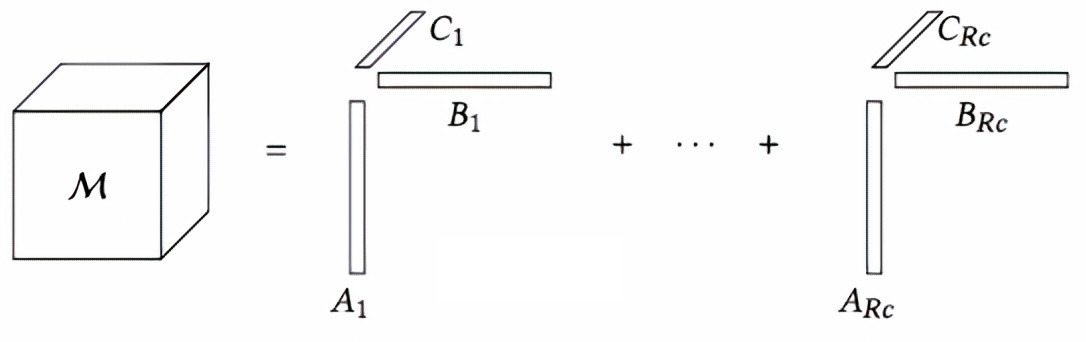
\includegraphics[scale=0.1, width=0.75\textwidth]{Dali2_ml_resize_x2.jpg}
                \begin{equation*}
                    \resizebox{0.25\textwidth}{!}{$
                    \small{\mathcal{M} = \sum_{r=1}^R A_r \circ B_r \circ C_r}$}
                \end{equation*}
            \end{center}
            
            \begin{equation*}
                min \ f(A, B, C) = \frac{1}{2}\|\mathcal{M} - [A, B, C]\|^2
            \end{equation*}
            \vspace*{2em}

            \begin{columns}[t]
                \begin{column}{.45\linewidth}
                    \textbf{Gradient:}
                        \begin{equation*}
                            \nabla \mathbf{f} = [
                                \mathsf{vec}(\frac{\partial f}{\partial A})^{\text T} \
                                \mathsf{vec}(\frac{\partial f}{\partial B})^{\text T} \
                                \mathsf{vec}(\frac{\partial f}{\partial C})^{\text T} \ ]^{\text T}
                        \end{equation*}
                        where
                        \begin{equation*}
                            \frac{\partial f}{\partial A} = -M_{(1)}(C\odot B) + A(C^{\text T} C\ast B^{\text T} B)
                        \end{equation*}
                \end{column}
                \begin{column}{.10\linewidth}
                \end{column}
                \begin{column}{.40\linewidth}
                    \textbf{Jacobian:}
                    \begin{equation*}
                        \mathbf{J} = [J_A \ J_B \ J_C]
                    \end{equation*}
                    where\\
                    \begin{equation*}
                        J_A = -(C\odot B) \otimes I_n
                    \end{equation*}
                \end{column}
            \end{columns}
        \end{block}
    \end{column}







    
    \begin{column}{.5\linewidth}
    \begin{block}{Modifying CPDGN to search for Cyclic Invariance}
            \textbf{Substitutions and Derivations:}
            \begin{center}
                $\mathbf{A} = \begin{bmatrix}
                    \mathbf{S} & \mathbf{U} & \mathbf{V} & \mathbf{W}\\
                \end{bmatrix}$\\
                $\mathbf{B} = \begin{bmatrix}
                    \mathbf{S} & \mathbf{W} & \mathbf{U} & \mathbf{V}\\
                \end{bmatrix}$\\
                $\mathbf{C} = \begin{bmatrix}
                    \mathbf{S} & \mathbf{V} & \mathbf{W} & \mathbf{U}\\
                \end{bmatrix}$
            \end{center}

            \begin{center}     
                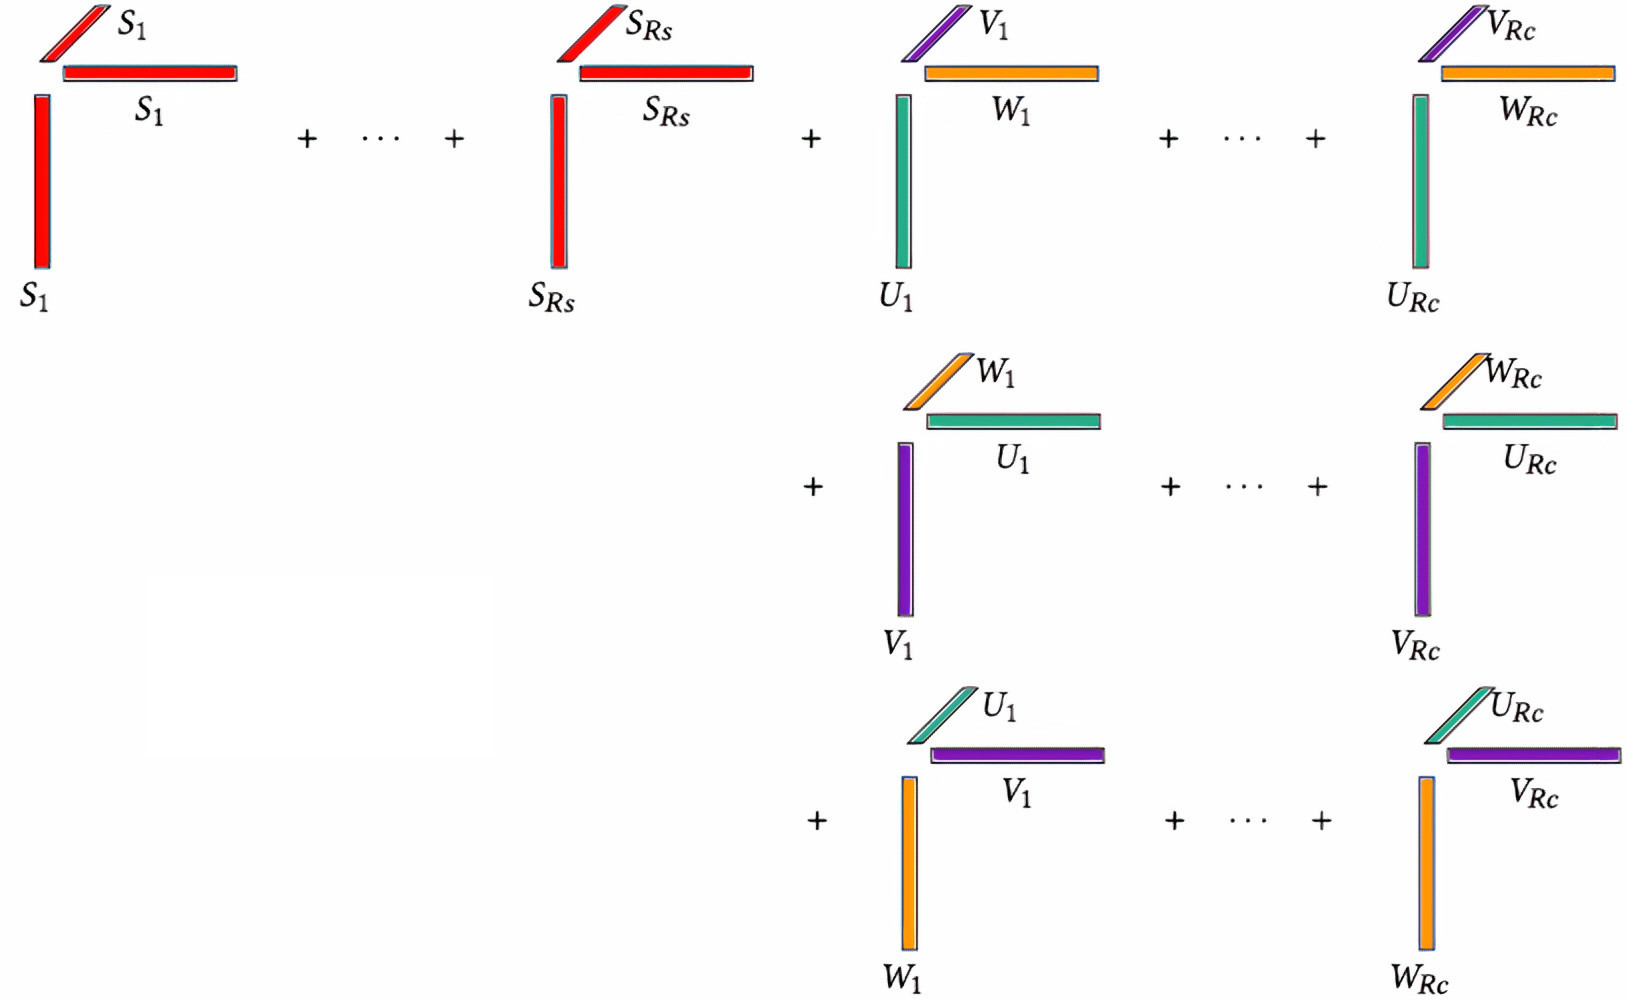
\includegraphics[scale=10, width=0.95\textwidth]{PicassoCo_ml_resize_x2.jpg}
                \begin{equation*}
                    \scalebox{0.9}{$
                    \small{\mathcal{M} = \sum_{q=1}^{Rs} S_q \circ S_q \circ S_q} + \sum_{k=1}^{Rc} (U_k \circ V_k \circ W_k + W_k \circ U_k \circ V_k + V_k \circ W_k \circ U_k)$} 
                \end{equation*}
            \end{center}

            \begin{equation*}
                    min \ f(S, U, V, W) = \frac{1}{2}\|\mathcal{M} - [S, S, S] - [U, V, W] - [W, U, V] - [V, W, U]\|^2
            \end{equation*}
            \textbf{Gradient:}
            \begin{equation*}
                            \nabla \mathbf{f} = [
                                \mathsf{vec}(\frac{\partial f}{\partial S})^{\text T} \
                                \mathsf{vec}(\frac{\partial f}{\partial U})^{\text T} \
                                \mathsf{vec}(\frac{\partial f}{\partial V})^{\text T} \
                                \mathsf{vec}(\frac{\partial f}{\partial W})^{\text T}]^{\text T}
                        \end{equation*}
            
            \begin{eqnarray*} 
                    \frac{\partial f}{\partial U} = & 3 \Bigl(S\bigl((S^{\text T} V)\ast (S^{\text T} W)\bigl)
                    + U\bigl((V^{\text T} V)\ast(W^{\text T} W)\bigl) \\
                    & + V\bigl((W^{\text T} V)\ast(U^{\text T} W)\bigl) 
                    + W\bigl((U^{\text T} V)\ast(V^{\text T} W)\bigl)\Bigl)\\ 
                    & - M_{(1)}(V\odot W) - M_{(2)}(W\odot V) - M_{(3)}(V\odot W) \\
            \end{eqnarray*}

            \textbf{Jacobian:}
            \begin{equation*}
                \mathbf{J} = 
                \begin{bmatrix}
                    J_s & J_u & J_v & J_w 
                \end{bmatrix}
                \in \mathbb{R}^{n^3\times n(R_s + 3R_c)}
            \end{equation*}

            \begin{equation*}
                J_u & = (V\odot W) \otimes I_n + \Pi_2^{\text T}\cdot (W\odot V) \otimes I_n + \Pi_3^{\text T}\cdot (V\odot W) \otimes I_n
            \end{equation*}

            \begin{equation*}
                J^{\text T} J \cdot vec(G) = 
                \begin{bmatrix}
                    J_s^{\text T} J_s & J_s^{\text T} J_u & J_s^{\text T} J_v & J_s^{\text T} J_w \\
                    J_u^{\text T} J_s & J_u^{\text T} J_u & J_u^{\text T} J_v & J_u^{\text T} J_w \\
                    J_v^{\text T} J_s & J_v^{\text T} J_u & J_v^{\text T} J_v & J_v^{\text T} J_w \\
                    J_w^{\text T} J_s & J_w^{\text T} J_u & J_w^{\text T} J_v & J_w^{\text T} J_w
                \end{bmatrix}
                \begin{bmatrix}
                    vec(G_s) \\
                    vec(G_u) \\
                    vec(G_v) \\
                    vec(G_w)
                \end{bmatrix}
            \end{equation*}

            \begin{eqnarray*}
                J_u^{\text T} J_svec(G_s) & = 3 vec\Bigl(G_s(S^{\text T} V)\ast (S^{\text T} W) + S\bigl((G_s^{\text T} W)\ast (S^{\text T} V) + (G_s^{\text T} V)\ast (S^{\text T} W)\bigl)\Bigl)
            \end{eqnarray*}           
        \end{block}

        
        \begin{block}{Preliminary Results}
        \textbf{Findings so far:}
            \begin{table}
              \centering
              \begin{tabular}{|c|c|c|}
                \hline
                $\mathcal{M}_2$ Rank 7 & $\mathcal{M}_3$ Rank 23 & $\mathcal{M}_4$ Rank 49\\
                \hline
                Rs=4, Rc=1 & Rs=11, Rc=4 & Rs=16, Rc=11 \\
                \hline
                Rs=1, Rc=2 & Rs=5, Rc=6 & Rs=1, Rc=16 \\
                \hline
                & Rs=2, Rc=7 & \\
                \hline
              \end{tabular}
              \caption{Exact Solutions through Cyclic Invariant CPDGN}
              \label{tab:simple_table}
            \end{table}
            There is also evidence for numerical solution in Rs=8, Rc=5 for $\mathcal{M}_3$ Rank 23 as well lower ranks. Additionally, there is evidence for several different Rs's for $\mathcal{M}_4$ Rank 49. 

        \newline\textbf{Future Work:}
        Explore the possibility of numeric solutions in places named above, as well as searching for lower ranks in $\mathcal{M}_4$ and bigger Matrix Multiplication Tensors.
        \end{block}
    \end{column}
\end{columns}
\begin{block}{References}
            \begin{enumerate}
                \item Rouse, Kathryn Z., and Grey M. Ballard. “On the Efficiency of Algorithms for Tensor Decompositions and Their Applications.” Wake Forest University, 2018. Print.
                \item G. Ballard, C. Ikenmeyer, J. Landsberg and N. Ryder, The geometry of rank decompositions of matrix multiplication II: 3x3 matrices, Journal of Pure and Applied Algebra, Volume 223, Number 8, pp. 3205 - 3224, 2018.
            \end{enumerate}
        \end{block}
\end{frame}
\end{document}
